% !TEX encoding = UTF-8 Unicode

\section{Sensorenhet}

Sensorenheten är den enhet som behandlar all sensordata. Den samlar in data från 
avståndssensorerna och linjesensorerna som den sedan antingen omvandlar till 
cm värden i avståndsensorns fall, eller trösklar och ger diskreta varierande storheter 
som i linjesensorns fall. Linjesensorn kommunicerar sedan med kommunikationsenheten
som förmedlar värdena till styrenheten och till PCn.

\subsection{Hårdvara}
Sensorenheten utgörs av en AVR microcontroller samt de analoga sensorer som är kopplade till denna. Sensorenheten består av en AVR ATmega16 som 
kopplats till fem avståndssensorer, de sensorer som hittar linjer på marken samt en display. För AD-omvandlig så används den interna omvandlaren på port A
i mikroprocessorn, se figur \ref{fig:PINsensor}. 

%Linjesensorer
Linjeföljarsensorn utgörs av en reflexsensormodul kopplad till en mux och en demux av typen 4067. Reflexsensormodulen består av 11 lysdioder och 11 ljuskänsliga transistorer. 

%Avståndssensorer
Sensorenheten har fem optiska avståndsmätare av typen \emph{GP2Y0A02YK} (20-150 cm). Två är placerade på vardera sida av roboten, en fram och en bak på var sida. Vidare sitter en sensor riktad framåt. 

%Display
En alfanumerisk LCD-display av typen \emph{LCD JM162A} används för att visa avstånd till väggarna när roboten är i labyrintläge. 


\begin{figure}[H]
  \centering
 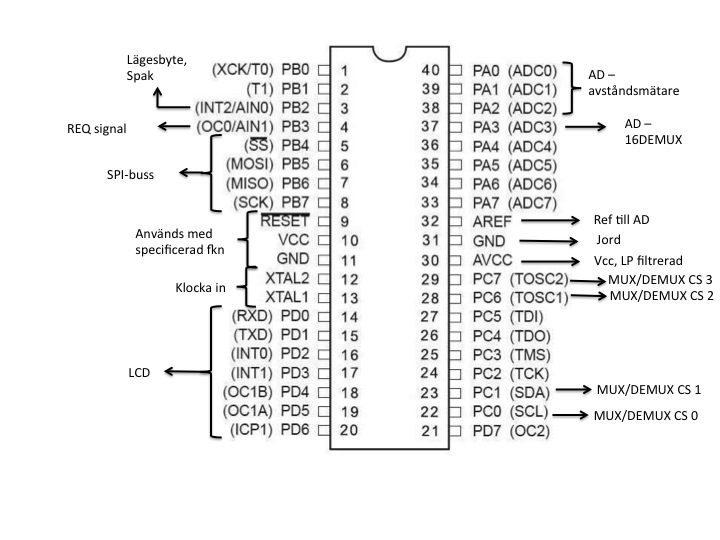
\includegraphics[angle=0,scale=0.5]{bilder/PIN_sensor.jpg}
  \caption{Sensorsenhetens pin-anslutningar}
  \label{fig:PINsensor}
\end{figure}

\subsubsection{Linjeföljarsensor}
För att maximera robotens framförhållning är sensorerna monterade framför roboten 
så långt fram som möjligt ca 3 mm ovanför marken. Linjesensorn består av 11st lysdioder 
med 11st ljuskänsliga transistorer, en multiplex och en demultiplex.

\begin{figure}[H]
  \centering
 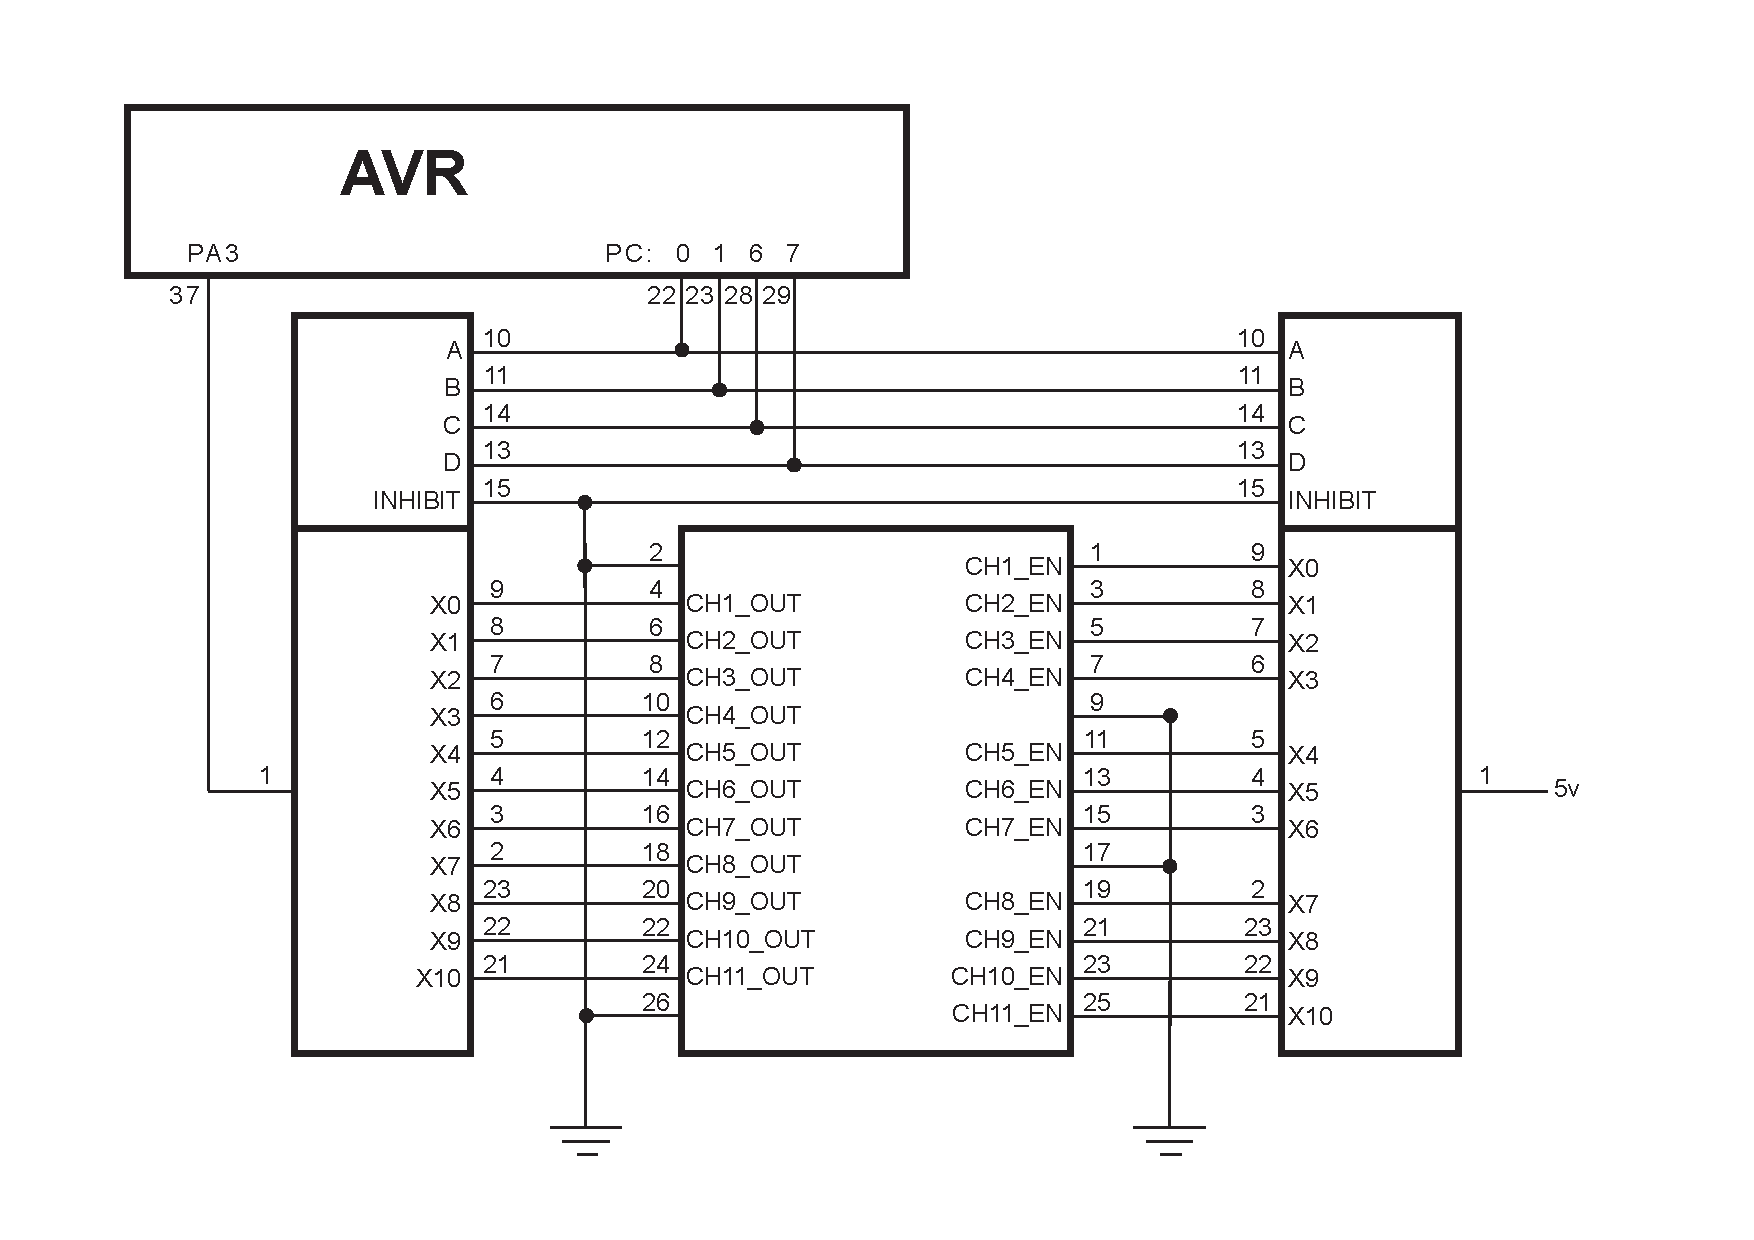
\includegraphics[angle=0,scale=0.5]{bilder/Uppkoppling_linjesensorer.pdf}
  \caption{Uppkoppling linjesensorer}
  \label{fig:Uppkoppling_linjesensorer}
\end{figure}


I Figur \ref{fig:Uppkoppling_linjesensorer} visas uppkopplingen av multiplexen och
demultiplexen  med linjesensorerna och AVRen. signalerna CH1 EN – CH11 EN 
är ingångar som leder signalen (logiskt 1) vidare till lysdioderna. 
CH1  OUT - CH11 OUT Leder svarssignalen från transistorerna vidare mot styrenhetens 
AVR. Multiplexen och demultiplexen styrs med signalerna A – D från AVRen. Inhibit 
signalen är jordad då dataväljning alltid ska vara tillåten.


\subsubsection{Avståndssensorer}
På roboten sitter fem avståndssensorer av typ GP2Y0A02YK som mäter avstånd
mellan 20 och 150 cm. Två sitter på robotens vänstra sida, två på högra och en
rakt fram. Dessa sensorer ger spänningsspikar varje millisekund så lågpassfilter
används för att få en jämnare signal utan spikar. Lågpassfiltren figur
har skärfrekvensen 54 Hz, se figur \ref{fig:lagpassfilter}. Utsignalen från
lågpassfiltrena är kopplade till port A på AVRen, se figur \ref{fig:PINsensor}.

\begin{figure}[H]
  \centering
 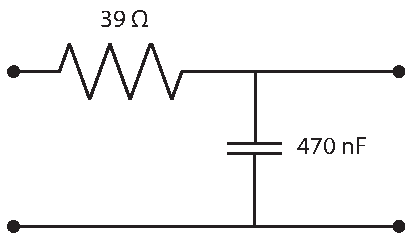
\includegraphics[angle=0,scale=0.7]{bilder/LPfilter.pdf}
  \caption{Lågpassfilter}
  \label{fig:lagpassfilter}
\end{figure}



\subsubsection{Display}
Robotens display-enhet är av typ \emph{LCD JM162A}. Displayen används för att 
visa avståndssensorernas värden. Eftersom sensorerna bara kan ge korrekta 
värden i intervallet 20-120 cm så kommer även displayen arbeta i detta 
intervall. Displayen arbetar i åtta databitarsläge och visar två rader med 
tecken. 

%Pinnar
Förutom de åtta databitarna som överförs för varje tecken till displayen så 
går ytterligare två signaler mellan sensorenhetens mikroprocessor och 
displayenheten: \emph{Enable} och \emph{Register select}. Enable-signalen 
signalerar till displayen att något ska skrivas ut, och Register select 
väljer mellan input-lägena 'data' och 'function'. Då det aldrig är någon data 
som läses från displayen så är pinnen \emph{R/W} konstant låg. 

%Kod
Sensorenheten har två funktioner som kan kallas för att skriva ut ett tecken 
på displayen. I funktionen \emph{char\_to\_display} anges parametrarna vilket 
tecken (givet i ASCII-kod) som ska skrivas ut, samt vilken position på 
displayen som ska skrivas till. Denna funktion används för bokstäver. För att 
skriva ut sensorvärden används funktionen \emph{data\_to\_display}, vilken 
tar parametrarna för sensorvärdet i cm samt vilken sensor som skickat det. 

Sensorprocessorn har också en funktion för att konvertera cm-värdet till ASCII
-kod, vilken används av \emph{data\_to\_display}.

\subsection{Mjukvara}

Mjukvaran i sensorenheten styr allt ifrån inläsning och tolkning av sensordata, fattar 
speciella styrbeslut om möjligt och upptäcker om något speciellt kommando behöver utföras.

Två viktiga funktioner i mjukvaran är AD-omvandlare, som omvandlar den analoga spänning
som levereras från avståndssensorerna till ett hexadecimalt tal, och kontrollen av linjesensorn
som skapar en array där det går att avläsa vilka sensorer som ser tejp.

\subsubsection{Avståndssensor}
Avståndssensorerna levererar en spänning som AD-omvandlas för att få någonting som går att
hantera digitalt. Avståndssensorerna avläses 30 gånger per sekund. På roboten finns två 
olika sorters sensorer; en sort för distanser mellan 20-120 cm och en för distanser mellan 4-26 cm.

Roboten har 7 stycken avståndssensorer:

\begin{itemize}
\item Två stycken långdistanssensorer på var sida av roboten
\item En kortdistanssensor på var sida av roboten
\item En långdistanssensor riktad framåt
\end{itemize} 

Avståndssensorerna används förutom att ta fram reglerdata då roboten befinner sig i en labyrint 
också till att under speciella omständigheter, t.ex. en 90\degree kurva, ta fram ett specialkommando
som skickas till styrenheten som då utför en förprogrammerad procedur.

\subsubsection{AD}
AD-omvandlaren startas av ett interrupt som genereras av overflow på en timer.
Detta overflow genereras ca var 32 ms och omvandlar alla sensorer. 
Ytterligare tio avbrott genereras med jämna mellanrum innan nästa overflow 
kommer. Dessa avbrott omvandlar endast linjesensorerna då de kan uppdateras
oftare än avståndssensorerna. När en AD-omvandling är klar ställs interna och 
externa muxar om för nästa ad-omvandling i funktionen \emph{mux\_control}. Efter 
det omvandlas det färdiga digitala värdet till data som skickas till
styrenheten.

\subsubsection{Linjesensor}
\label{sec:linjesensor}
Styrsignaler till multiplexern väljer ut en diod i taget.
Varje diod på linjesensorn A/D-omvandlas och jämförs med ett tröskelvärde. Om
det omvandlade värder är
ett högt värde antas en tejp och en etta skiftas in i en byte och är det 
ett lågt värde så antas ingen tejp och en nolla skiftas in, varje diod
representeras alltså med en bit. Då det finns elva dioder så används två byte 
för att representera hela linjesensorn. Tröskelvärdet går att justera från PCn. 
Ur de två byten med linjedata räknas vilket index som tejpen befinner sig på,
detta indexet tar värden i intervallet 1-11. Från indexet beräknas en
reglerparameter, negativ om roboten är till vänster och positiv om den är till
höger. Denna parameter skickas till styrenheten där den används i
linjeregulatorn, se \ref{sec:linjereglering}. Linjedatat undersökts också efter
stoppsignaler i linjeläge och riktningsmarkeringar i labyrintläge.

\subsubsection{Upptäckning av riktningsmarkeringar}
\label{sec:riktmark}
Då roboten är i en labyrint kommer linjeföljarsensorn användas 
för att hitta riktningsmarkeringar. Dessa markeringar används för att visa i 
vilken riktning roboten ska färdas i nästkommande korsning.  I enlighet med 
banspecifikationen är funktionen anpassad för att uppfatta 
följande signaler:

Högersväng visas med en tunn tejpmarkering följd av en tre gånger så tjock.
Vänstersväng visas genom en tjock tejpmarkering följd av en tre gånger så tunn.
Framåt visas genom två tunna tejpmarkeringar. Se figur \ref{fig:tejpmarkeringar}.
för samtliga markeringars utseende.

\begin{figure}[H]
  \centering
 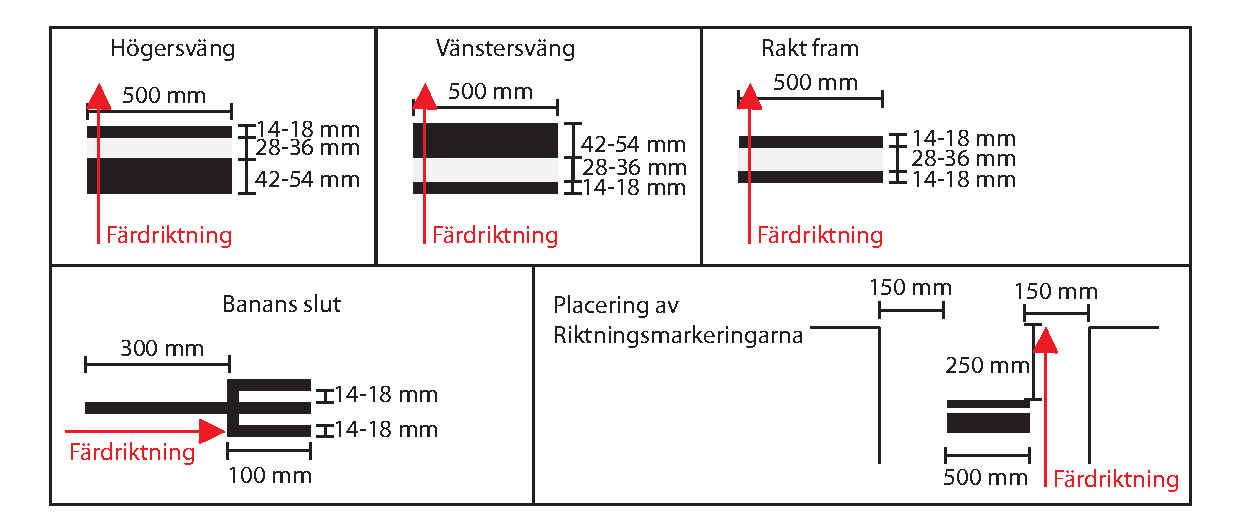
\includegraphics[angle=0,scale=0.5]{bilder/tejpmarkeringar.pdf}
  \caption{De olika typer av tejpmarkeringar som används}
  \label{fig:tejpmarkeringar}
\end{figure}


Vid varje uppdatering av samtliga linjeföljarsensorer görs en kontroll om de 
tre mittersta sensorerna ligger över tejp. Är så fallet så börjar antalet 
gånger linjesensorerna uppdateras att räknas. När de tre mittersta sensorerna 
inte längre ligger över tejp sparas antalet iterationer som sensorerna 
tillbringat över tejpen. Proceduren upprepas därefter och antalet iterationer 
jämförs för att se vilken tejpbit som var bredast, den första eller den andra
. Resultatet sparas därefter och efterfrågat kommando utförs i nästkommande 
korsning, se \ref{sec:upptackkorsning}.

\subsubsection{Upptäckning av stoppsignal}
När banan tar slut ska det i enlighet i banspecifikationen finnas en speciell typ av 
markering. Avslutet ska ske på en linje och markeringen går att se i figur \ref{fig:tejpmarkeringar}.
Robotens kommer att uppfatta markeringar där det finns mer än 5 distinkta skillnader mellan tejp och golv, förutsatt att den ser markeringen under en tidsperiod, som en stoppsignal. 

\subsubsection{Avståndsberäkning}
Då alla avståndssensorer är individer, det vill säga de levererar inte samma spänningar vid
samma avstånd, så behövs det en normering av värdena till centimeter för att kunna reglera
på sensordatan. 

Avstånden i centimeter ska också skickas till datorn och displayen, i enlighet med
kravspecifikationen.

På roboten används två olika sorters avståndsensorer, en sort för längre sträckor och en sort för
kortare sträckor. De sensorer som klarar av längre sträckor fungerar mellan 20-150 cm men 
används bara i intervallet 20-120 cm. De sensorer som är till för kortare distanser fungerar mellan 4-30 cm,
 men används bara mellan 4-26 cm. Samtliga avståndssensorer är icke-linjära, det vill säga att de 
 inte levererar en spänning som är linjärt proportionerlig mot avståndet.

Detta har lösts genom att varje sensors hexadecimala utvärde, efter AD omvandlingen, linjäriseras i minst 
tre olika intervall.

\subsubsection{Upptäckning av korsningar och 90\degree svängar}
\label{sec:upptackkorsning}
Enligt specifikationen av den bana som roboten ska kunna följa, framgår det 
att det före alla korsningar ska finnas tejpmarkeringar som visar i vilken 
riktning roboten ska svänga, se \ref{sec:riktmark}. Roboten kommer att 
upptäcka korsningar om två eller fler av riktningarna höger, vänster och framåt visar 
mer än 80 cm.

Roboten kommer att upptäcka 90\degree svängar om det är längre än 80 cm åt 
höger eller vänster(inte båda), samt mindre än 35cm framåt.

Upptäcker roboten en korsning kommer det kommando som beskrivits av tidigare 
tejpmarkeringar att skickas till styrenheten. Det data som skickas är skrivet 
för att uppfattas som ett så kallat specialkommando, det vill säga 
styrenheten har en procedur som utförs utan att ta hänsyn till den reglerdata 
som skickas från sensorenheten. Märk att detta specialkommando innehåller en 
framkörning till mitten av korsningen, till skillnad från 90\degree svängar 
som utförs omedelbart.

Upptäcker roboten en 90\degree sväng kommer ett annat specialkommando att 
utföras, där roboten svänger 90\degree åt det håll som avståndssensorerna 
visar har det längre avståndet.

\begin{itemize}
\item Långdistanssensorerna är linjäriserade för intervallen 20-40 cm, 41-60 cm och 61-120 cm
\item Kortdistanssensorerna är linjäriserade för intervallen 4-7 cm, 8-12 cm och 13-26 cm
\end{itemize}
 

För samtliga grafer för linjäriseringen, se appendix \ref{appendix:cmomvandling}.


\subsubsection{Kommunikation}
Kommunikationsenheten använder den anslutna databussen för att förmedla 
data till andra delar av roboten. Sensorenheten är den stora leverantören av 
data i systemet och sänder iväg betydligt mer data än vad den tar emot. För att 
adressera och specificera den data som skickas iväg från sensorenheten märks 
headerbyten upp med diverse olika flaggor och adresseringsbitar. För mer info om 
dessa, se \ref{sec:protokoll}. Den enda data som tas emot av sensorenheten är en 
referenskod för att kalibrera linjesensorerna.

I fjärrstyrt läge så skickar sensorenheten avståndet från avståndssensorerna 
till datorn.  I detta läge skickar sensorenheten ingen data till styrenheten. 
I autonomt läge då roboten befinner sig över en linje skickar sensorenheten data om 
var tejpen befinner sig på linjesensorn till styrenheten, samt avståndet till 
väggarna till datorn. Befinner sig roboten i en labyrint skickar 
sensorenheten avståndet till väggarna till både sensorenheten och datorn.  

Då sensorenheten tar ett beslut om att ett avvikande beteende är nödvändigt, till exempel 
en korsning eller en stoppmarkering, så skickas denna information alltid till 
både styrenheten och datorn.


